\hypertarget{objectives-and-challenges}{%
\chapter{Objectives and Challenges}\label{objectives-and-challenges}}

\begin{itemize}
  \item What is the likeliness for two target signals being overlapped for different scenarios
  \item Unison
  \item past research was focused on solving source separation because its such an interesting and challenging mathematical problem. Data driven separation, however, changed this.
\end{itemize}

In the previous chapter, I introduced the basic signal processing fundamentals in the context of audio mixtures and typical tasks and applications.
In this chapter I want to point out possible objectives and challenges that were the basis for the work that was carried out for this thesis as possible future research that this work might have enabled.

\hypertarget{highly-overlapped-signals}{%
\section{The Case of Highly Overlapped Signals}\label{highly-overlapped-signals}}

% from zafar >> rewrite!
A TF representation is typically used as a first step in processing the audio because sources tend to be less overlapped in the TF representation than in the waveform~\cite{rickard02, giannoulis11}.
E.g. a STFT can be used as it can allows for easy reconstruction of the original waveform and provides a good trade-off between computational complexity and overlap.
The TF representation makes it easier to filter the mixture that correspond to only a single source.
% todo check where this is from
The focus of many source separation methods is to extract individual by modeling their respective target in the non-negative
time-frequency domain.
%check
For many separation scenarios this is a reasonable approach as it is usually assumed that the time-frequency-domain (STFT) provides sufficient level of separability (e.g.~by given a perfect mask).
The actual extraction or filtering is then done by synthesizing the estimate of the model and applying the originals mixture phase.
Often the assumption here is that the mixture representation allows to apply filtering in a way that sufficiently extracts all targets from the mixture.
\\

In practice this depends on the amount of overlap of the sources.
A small amount of overlap can be tolerated to still sufficiently extract the sources.
If sources are fully overlapped a separation in the TF domain is hardly possible.
The separability of sources in the time frequency domain can be measured as it has been done in~\cite{rickard02, giannoulis11}.
% check
In linear mixtures, \emph{separability} is defined as a measure that indicates the percentage of time-frequency bins of a source is disjoint from those of interfering sources.
An extensive study using this W-disjoint orthogonality metric (WDO) is given in~\cite{rickard02}.
If \(M\) is the ideal binary mask for a given target \(S\) and it's interfering
magnitude model \(Y\), \(WDO\) is defined as:

\begin{equation}
    PSR_{M} = \frac{\|M \cdot S_{k}\|^{2}}{\|S_{k}\|^{2}}
\end{equation}

\begin{equation}
    SIR_{M}=\frac{\|M \cdot S_{k}\|^{2}}{\|M \cdot Y_{k}\|^{2}}
\end{equation}

\begin{equation}
    WDO_{M} = PSR_{M} - \frac{PSR_{M}}{SIR_{M}}
\end{equation}

%Ideal Ratio Mask:
%\(\hat{\mathbf{x}}=\frac{\mathbf{v_j}}{\sum_{j'=1}^{J}\mathbf{v}_j'}\mathbf{x}\)

A \(WDO\) of one means the sources are perfectly disjoint, hence no overlap.
A \(WDO\) zero means can be interpreted as sources being fully overlapped.
So we identify an important aspect which is the levels of overlap in the context of audio sources.
In the past many research has been focused on separation and analysis of mixtures in various scenarios.
Two scenarios remain to be very popular for the reason of either large amount of applications or the number of available data samples:

\begin{description}
  \item[Cocktail Party:] Here, multiple speakers are active at the same time (concurrent).
  Due to the fact that concurrent speakers are speaking the same sentences, it results in an overlap of speech signals in both time an frequency.
  \item[Vocal Accompaniment Separation:] In music separation this is one of the most popular separation tasks with a large number of contributions~\cite{rafii18}.
  Usually the assumption is that the vocals is more sparse whereas the accompaniment is more stationary.
\end{description}

For music signals, the type of instrument is important for the amount of overlap.
Furthermore, both scenarios depend on the number of sources, e.g. imagine a cocktail party of ten concurrent speakers speaking with same amplitude level.
This is similar to music where the overlap can range from two instruments with very different characteristics like guitar and drums, to two instruments playing the same note (unison).\\

\begin{figure*}[h]
\centering
\subcaptionbox[Speech]{Speech}%
[1\textwidth]{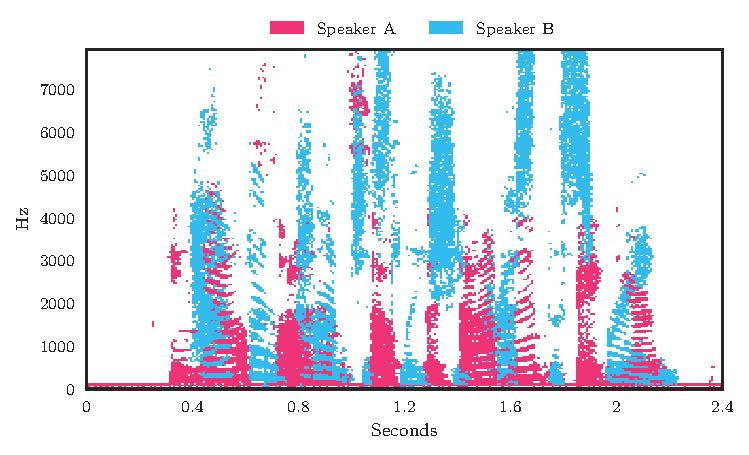
\includegraphics[width=0.8\textwidth]{gfx/dominance_map_speakers.pdf}}%
\hspace{0.2\textwidth} % seperation
\subcaptionbox[Vocal/Accompaniment]{Vocal/Accompaniment}
[1\textwidth]{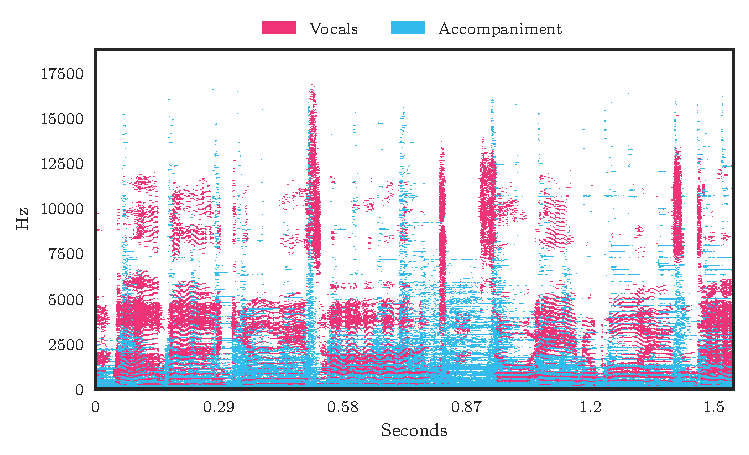
\includegraphics[width=0.8\textwidth]{gfx/dominance_map_vocacc.pdf}}%
\hspace{0.2\textwidth} % seperation
\subcaptionbox[Speech]{Unsison}
[1\textwidth]{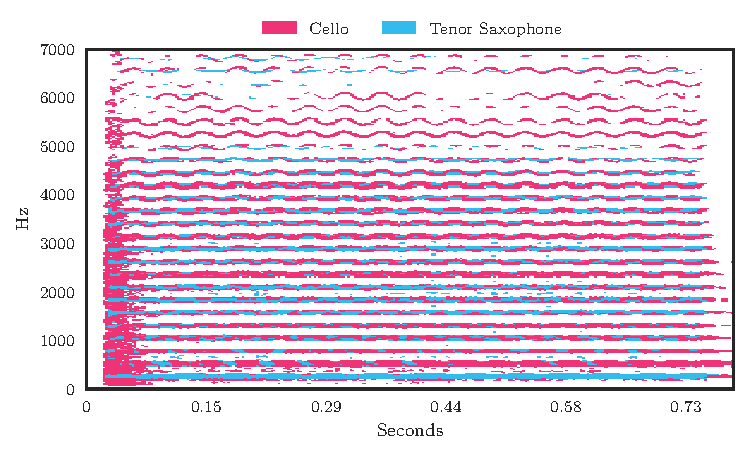
\includegraphics[width=0.8\textwidth]{gfx/dominance_map_unison.pdf}}%
\caption{Predominant source activity, showing the predominant source for each time frequency entry. Computed using binary masks of each source entry.}
\label{fig:dominance}
\end{figure*}

\begin{figure*}[h]
\centering
\subcaptionbox[Speech]{Speech}%
[1\textwidth]{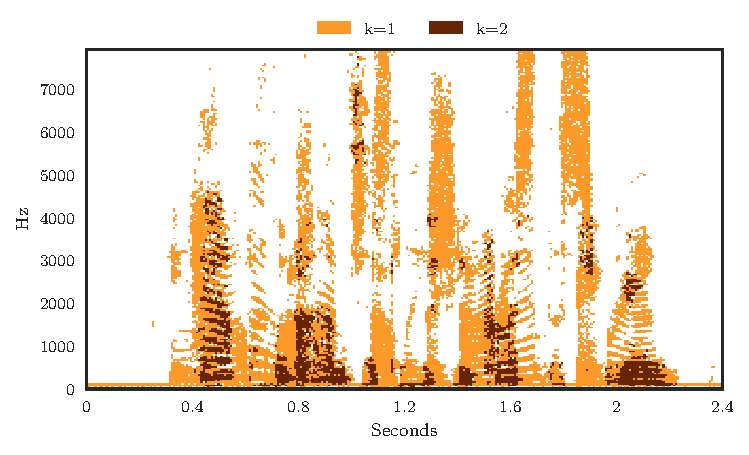
\includegraphics[width=0.8\textwidth]{gfx/count_map_speakers.pdf}}%
\hspace{0.2\textwidth} % seperation
\subcaptionbox[Vocal/Accompaniment]{Vocal/Accompaniment}
[1\textwidth]{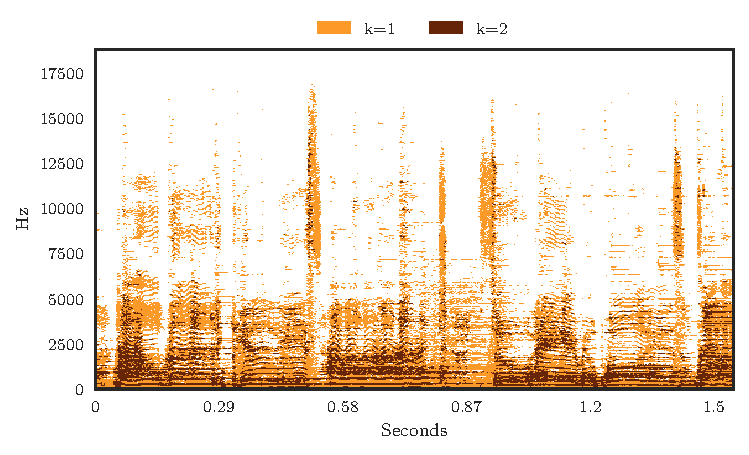
\includegraphics[width=0.8\textwidth]{gfx/count_map_vocacc.pdf}}%
\hspace{0.2\textwidth} % seperation
\subcaptionbox[Unison]{Unison Instruments}
[1\textwidth]{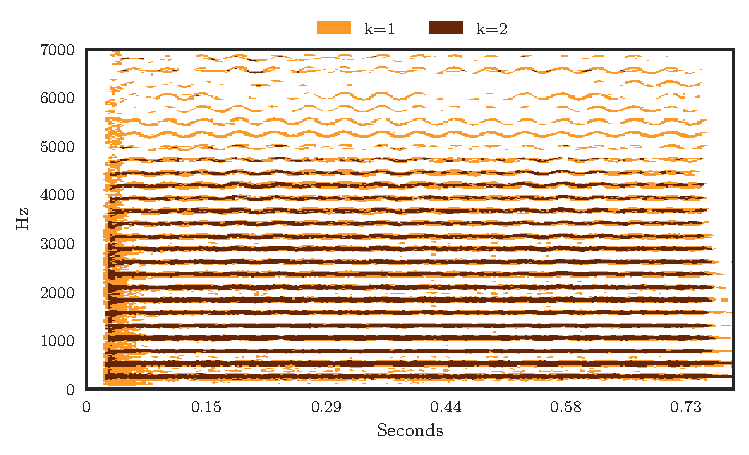
\includegraphics[width=0.8\textwidth]{gfx/count_map_unison.pdf}}%
\caption{Source Count Activity showing the number of sources $k$ for each time frequency entry. Computed using binary masks of each source entry.}
\label{fig:count}
\end{figure*}


I depict spectrogram examples these scenarios in Figures~\ref{fig:dominance} and~\ref{fig:count}.
The figure shows the the number of TF entries that predominantly belong to either one of the two source classes.
Also it shows for each TF entry the number of active sources.
From this plot one can see that the overlap of a typical speech mixture is comparable to a music recording where the task is to separate vocals and accompaniment.\\

If we compare this to a scenario where sources are fully overlapped as in Figure~\ref{fig:unison_count} we can see that almost all TF bins are overlapped and separation will hardly be possible.
In a small experiment, I computed the average \(WDO\) for random 1000 mixtures of each scenario~\footnote{Please see details in Chapter~\ref{X}}.
It turned out that for speech separation of \(k=2\) speakers, \(WDO=0.9\) and for the vocal accompaniment scenario \(WDO=0.87\), which is surprisingly similar even though both scenarios are so fundamentally different.
In the case of the two instruments playing in unison the average WDO is \(0.65\), hence a good separation in the time frequency domain is barely possible.
While this is an extreme scenario, it provides a case where typical assumptions are violated and it would facilitate the demand to develop new methods that do not rely so much on these long standing assumptions.
\\
In fact, coming up with an idea for a method that could separate the example of Figure~\ref{fig:unison_count} is possible by just looking closely at the spectrograms of Figure~\ref{X}.
We see that the slow spectro-temporal modulations caused by the vibrato is one of the aspects where the two sources differ significantly.
So instead of a TF representation, one would need to pick a representation that allows to separate the two sources in their modulation domain.
In audio long term modulations or spectral temporal variations of mixtures has not yet been studied well.
Therefore, I want to focus on these modulational aspects on mixtures in the next section.

\hypertarget{research-track-modulations}{%
\section{Research track: Slow Modulation}\label{research-track-modulations}}

Modulations occur both in speech and music signals and is usually a combination between amplitude and frequency modulation.
%lets start with speech
In speech, techniques to utilise spectro-temporal modulation patterns in processing enables further applications such as~\cite{mesgarani04} or extract spatial acoustic signatures from mixtures~\cite{sukittanon06}.
Is also shown that it can improve speech intelligibility~\cite{elhilali03} or automatic speech recognition~\cite{kingsbury98}.

% now go to music, TODO: check papers by in ewert and driedger
In music, vibrato is an effect that is well studied especially in musicology~\cite{A, B, C, D, E}.
Performers of musical to perform a vibrato in the same way when repeating a performance. This can be exploited in
source separation scenarios.
Typically, vibratos have modulation frequencies (rates) which vary between 4 and 8 Hz which is magnitudes slower compare to the actual fundamental frequency of the source.
Additionally vibrato rates vary across different instruments.
In~\cite{macleod2006} the vibrato width (frequency deviation) was found to be significantly different between violinists and violists performers.\\

\subsection{Perception}
There are indications that humans use modulations to segregate sounds as well~\cite{dau99}.
Humans make use of the concept of Common Amplitude Modulation~\cite{bregman90} to segregate sources in mixture.
CAM is effectively the property of harmonics that share the
same amplitude modulation across the bins.

\subsection{Representations}
One way of analysing amplitude modulations is to use a modulation spectrogram~\cite{greenberg97} which is a frequency-frequency
representation of a time domain input signal.
A complete signal representation can be archived by a modulation tensor which holds the modulation spectrograms for each time frame.
For further details the reader is referred to~\cite{barker15}.

\subsection{Modulations for Processing Mixtures}
There exist a number of method that utilise spectro-temporal modulation to process or separate mixtures.

% from zafar!
Wang proposed instantaneous and frequency-warped techniques for signal parameterization and source separation, with application to voice separation in music~\cite{wang94,wang95}.
He introduced a frequency-locked loop algorithm which uses multiple harmonically constrained trackers.
He computed the estimated fundamental frequency from a maximum-likelihood weighting of the tracking estimates. He was then able to estimate harmonic signals such as voices from complex mixtures.\\
% from zafar
Wolf et al. proposed an approach using rigid motion segmentation, with application to singing voice separation \cite{wolf14,wolf16}. They introduced harmonic template models with amplitude and pitch modulations defined by a velocity vector. They applied a wavelet transform \cite{anden14} on the harmonic template models to build an audio image where the amplitude and pitch dynamics can be separated through the velocity vector. They then derived a velocity equation, similar to the optical flow velocity equation used in images \cite{bernard01}, to segment velocity components. Finally, they identified the harmonic templates which model different sources in the mixture and separated them by approximating the velocity field over the corresponding harmonic template models.\\
% from zafar
Yen et al. proposed an approach using spectro-temporal modulation features \cite{yen14,yen15}. They decomposed a mixture using a two-stage auditory model which consists of a cochlear module \cite{chi05} and cortical module \cite{chi99}. They then extracted spectro-temporal modulation features from the TF units and clustered the TF units into harmonic, percussive, and vocal components using the EM algorithm and resynthesized the estimated signals.\\
% from zafar
% double check this!
Usage for source separation, non FM modulations are considered: \cite{hennequin10}.
An advantage of the source-filter model approach is indeed that one can dissociate the pitched content of the signal, embodied by the position of its harmonics, from its TF envelope which describes where the energy of the sound lies. In the case of vocals, it yields the ability to distinguish between the actual note being sung (pitch content) and the phoneme being uttered (mouth and vocal tract configuration), respectively. One key feature of vocals is they typically exhibit great variability in fundamental frequency over time. They can also exhibit larger \textit{vibratos} (fundamental frequency modulations) and \textit{tremolos} (amplitude modulations) in comparison to other instruments.
% from zafar
Modeling the common amplitude modulation to separate mixtures has already been done in~\cite{li07} and
\cite{cano14}, which additionally included common amplitude modulation characteristics in the separation scheme.

\section{Objectives}

Even though modulations were already part of many scientific activities, I understand that there are still many open issues regarding the analysis and processing of these specific signals.
Therefore I identfy the following objectives as the basis for the contributions I made during this thesis.
\begin{description}
  \item[Scenarios and Datasets:] One of the objectives here is develop a new scenario where sources are highly overlapped such   as unison instruments or a large number of concurrent speakers. Also I envision scenarios where slow modulations can be      exploited. However generally data often is not available. Therefore one objective of this thesis is investigate the          creation new real and synthetic datasets.
  \item[Representations:] Highly overlapped signals require better representations, because separability is of highly overlapped source with modulations is sufficiently possible in the TF domain.
    Many of the representations require a parametric approach. And the existing modulation tensor is only able to capture amplitude modulation, hence it cannot solve general modulations.
    An objective of this thesis is to study representations that allow to analyse mixtures to improve separation.\emph{Chapter~\ref{X}}
  \item[Processing Methods:] Objective is to develop new methods to address the source separation scenario. These methods would be designed for the constrained scenarios where modulational effects can easily be exploited.
  \item[Generalisibility:] The goal then is to transfer the results and insights gained by these
    studies onto simpler scenarios to measure the actual effect.
  \item[Number of Sources:] Finally, in the context of source seperation of highly overlapped signals, an estimation of the number of sources is valuable. As very little research has been done in this direction, I want to investigate new methods to address the task of estimating the number of sources in highly overlapped mixtures.
\end{description}

In the next two chapters, I will present methods and arguments to address these objectives.

% TODO: add deep learning